\section{What is an \ab{} workflow system?}

\subsection{What are \ab{} calculations?}

\begin{frame}{What are \ab{} calculations?}
    \begin{definitionblock}{\ab{} calculation}
        A method of calculating atomic and molecular structure directly from the first
        principles of quantum mechanics, without using quantities derived from experiment
        as parameters.
    \end{definitionblock}

    \begin{itemize}
        \item Electronic structure computation
        \item Optimize input crystal/molecular structures
        \item Phonon vibrational spectra computation
        \item Helmholtz free energy calculation at finite temperature
        \item Linear elastic constants
        \item More...
    \end{itemize}
\end{frame}

\begin{frame}{Typical \ab{} workflows used in our group}
    \begin{figure}[H]
        \centering
        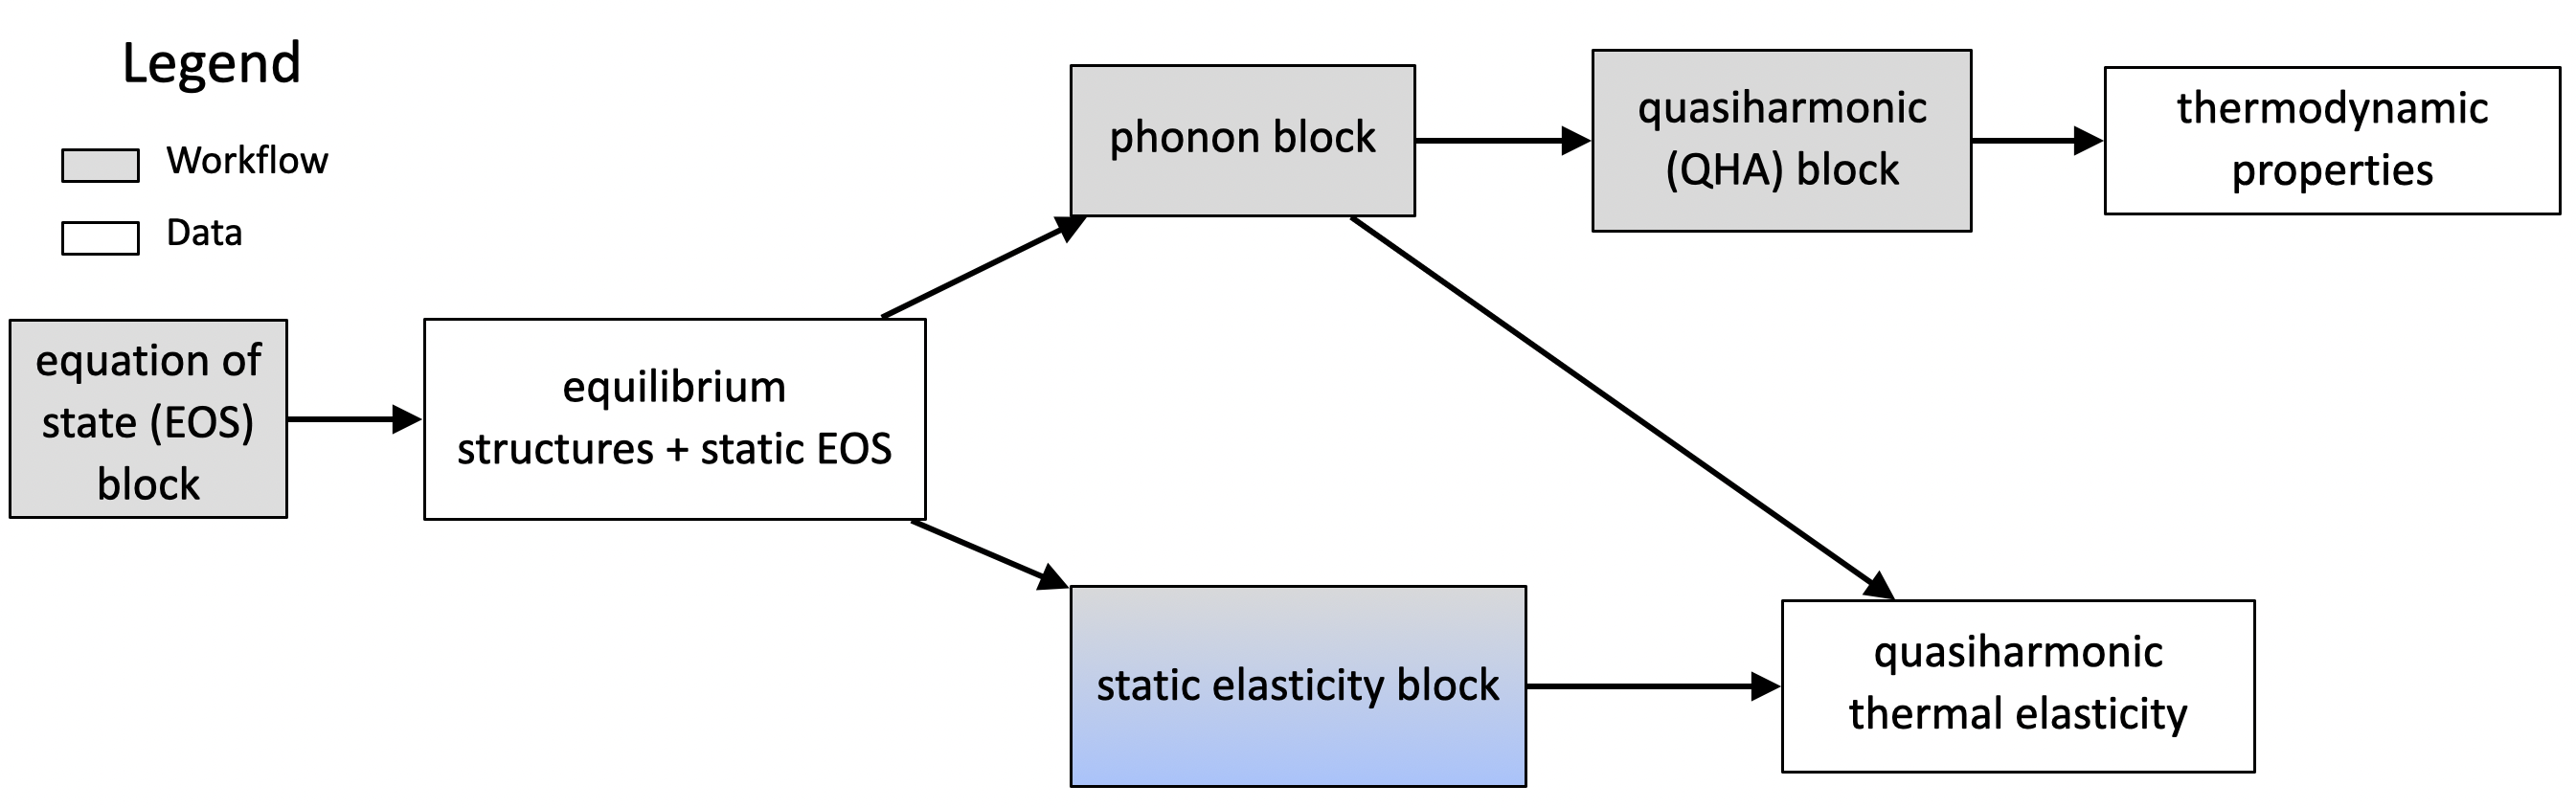
\includegraphics[height=0.4\textheight]{workflows}
        \label{eq:workflows}
    \end{figure}
\end{frame}

\begin{frame}{Various \ab{} software}
    To do \ab{} calculations, it is inevitable to interact with \ab{} software.
    There are a lot of them on the market, e.g., \qe{}, VASP, and ABINIT.
    They are often written in Fortran, and needed to be compiled to executable
    when using.

    So building a workflow for them requires us to create parsers for their input and output
    files, as well as functions to dynamically run these executables.

    \begin{figure}[b]
        \centering
        
\includegraphics[width=0.4\textwidth]{qe}
        \hfill
        
\includegraphics[width=0.2\textwidth]{vasp}
        \hfill
        
\includegraphics[width=0.3\textwidth]{abinit}
        \label{fig:abinitsoftware}
    \end{figure}
\end{frame}
\subsection{What is needed in an \ab{} workflow system?}

\begin{frame}{What is needed in an \ab{} workflow system?}
    There are at least three components:

    \begin{itemize}
        \item Sciency, technical stuff: calculations, input generation, output analysis...
        \item Dispatcher, job scheduler: interacting with \ab{} software, \texttt{mpi}...
        \item User interface: interacting with users
    \end{itemize}
\end{frame}

\subsection{What is \express{}?}

\begin{frame}{What is \express{}?}
    \begin{definitionblock}{\express{}}
        A workflow framework consisting of several extensible, lightweight, high-throughput,
        high-level Julia packages that aims to automate \ab{} calculations for the materials
        science community.
    \end{definitionblock}

    \begin{definitionblock}{\texttt{Express.jl}}
        The core package of the \express{} project, which manages and dispatches the rest
        packages in \express{}.
    \end{definitionblock}
\end{frame}
